\documentclass[a4paper, 12pt]{article}
\usepackage[utf8]{inputenc}
\usepackage[warn]{mathtext}
\usepackage[russian]{babel}
\usepackage[T2]{fontenc}
\usepackage[warn]{mathtext}
\usepackage{caption}

\usepackage{graphicx}
\graphicspath{ {images/} }
\usepackage{tikz}
\usepackage{pgfplots}

\usepackage{amsmath}
\usepackage{floatflt}
\usepackage[left=20mm, top=20mm, right=20mm, bottom=20mm, footskip=10mm]{geometry}

\usepackage{multicol}
\setlength{\columnsep}{2cm}


\usepackage{multicol}
\setlength{\columnsep}{2cm}
\usepackage{hyperref}

\begin{document}
	
\begin{titlepage}
	\centering
	\vspace{5cm}
	{\scshape\LARGE Московский физико-технический институт \par}
	\vspace{4cm}
	{\scshape\Large Лабораторная работа 4.3.4 \par}
	\vspace{1cm}
	{\huge\bfseries Метод преобразования Фурье в оптике \par}
	\vspace{1cm}
	\vfill
\begin{flushright}
	{\large выполнил студент 924 группы ФОПФ}\par
	\vspace{0.3cm}
	{\LARGE Панферов Андрей}
\end{flushright}
	

	\vfill

% Bottom of the page
	Долгопрудный, 2021 г.
\end{titlepage}

\paragraph*{Цель работы:} Исследовать явления дифракции Френеля и Фраунгофера на щели, изучить влияние дифракции на разрешающую способность оптических приборов.
\paragraph*{В работе используются:} Гелий-неоновый лазер, кассета с набором
сеток разного периода, щель с микрометрическим винтом, линзы,
экран, линейка.
$$$$
Анализ сложного волнового поля во многих случаях целесообразно проводить, разлагая его на простейшие составляющие, например, представляя его в виде разложения по плоским волнам. При этом оказывается, что если мы рассматриваем поле, полученное после прохождения плоской монохроматической волны через предмет или транспарант (изображение предмета на фотоплёнке или стеклянной пластинке) с функцией пропускания t(x), то разложение по плоским волнам соответствует преобразованию Фурье от этой функции. Если за предметом поставить линзу, то каждая плоская волна сфокусируется в свою точку в задней фокальной плоскости линзы. Таким образом, картина, наблюдаемая в фокальной плоскости линзы, даёт нам представление о спектре плоских волн падающего на линзу волнового поля. Поэтому можно утверждать, что с помощью линзы в оптике осуществляется пространственное преобразование Фурье.

\section*{Определение ширины щели}
\label{section_I}
\subsection*{Экспериментальная установка}

Схема установки представлена на рис. \ref{fig:scheme_I}. Щель переменной ширины D, снабжённая микрометрическим винтом В, освещается параллельным пучком света, излучаемым лазером (радиус кривизны фронта волны велик по сравнению с фокусными расстояниями используемых в схеме линз).

\begin{figure}[h]
    \centering
    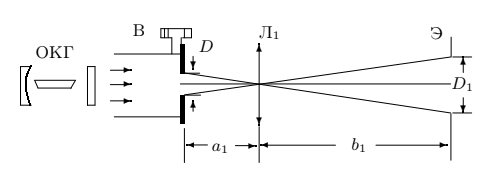
\includegraphics[width=15cm]{scheme_I.png}
    \caption{Схема лабораторной установки для определения ширины щели}
    \label{fig:scheme_I}
\end{figure}

Увеличенное изображение щели с помощью линзы Л1 проецируется на экран Э. Величина изображения D1 зависит от расстояний от линзы до предмета — $a_1$ и до изображения — $b_1$, т. е. от увеличения $\Gamma$ системы:

$$\Gamma=\frac{D_{1}}{D}=\frac{b_{1}}{a_{1}}$$

\newpage

\subsection*{Измерения}

\begin{enumerate}
    \item Соберем схему с Рис. \ref{fig:scheme_I}, используя короткофокусную линзу $F_3 = 3.8$ см.
    \item Определим начало открытия щели: $pos_0 = 0.50$ мм
    \item Меняя ширину щели от 50 до 500 мкм (5–50 делений от нового ну-
ля), снимем зависимость размера изображения $D1$ от ширины щели $b$ и занесем результаты в Таблицу \ref{table::size}. Построим график этой зависимости и по нему найдем увеличение $\Gamma_{graph} = 30 \pm 6$ и точный момент открытия щели $b_{I} = 0.62mm$ 

    \begin{minipage}{0.3\textwidth}
        \begin{tabular}{|ll|}
        \hline
        \multicolumn{1}{|l|}{$b$, мм} & $x$, мм \\ \hline
        0                             & 0       \\ \hline
        0.05                          & 3       \\ \hline
        0.1                           & 2.5     \\ \hline
        0.15                          & 1       \\ \hline
        0.2                           & 2       \\ \hline
        0.25                          & 3.5     \\ \hline
        0.3                           & 5       \\ \hline
        0.35                          & 6.5     \\ \hline
        0.4                           & 8       \\ \hline
        0.45                          & 10      \\ \hline
        0.5                           & 11      \\ \hline
        \end{tabular}
        \captionof{table}{Ширина щели и размер изображения}
        \label{table::size}
    \end{minipage}
    \begin{minipage}{0.7\textwidth}
        \begin{center}
            \begin{tikzpicture}[scale=1]
                \begin{axis}[
                    	axis lines = middle,
                    	xlabel = {$b$, мм},
                        ylabel = {$x$, мм},
                    	ylabel style={red, scale=1},
                        xlabel style={red, scale=1},
                    	title={Зависимость размера изображения от ширины щели},
                    	table/col sep=semicolon,
                    ]
            	    \addplot +[blue, only marks] plot[
        			error bars/.cd,
        			x dir = both,
        			x fixed = 0.01,
        			y dir = both,
        			y fixed = 1,
        		    ] table[x=B, y=X]{size.csv};
        		    \addplot[color=red, domain=0.1:0.5]{29.76 * x - 3.79};
            	\end{axis}
            \end{tikzpicture}
        \end{center}
    \end{minipage}


    \item Измерим расстояния $a_1 = 56 \pm 3$ мм и $b_1 = 119 \pm 1$ см. По ним вычислим $\Gamma_{lens} = 21.3 \pm 1.2$
\end{enumerate}

\section*{Определение ширины щели по её спектру}

\subsection*{Экспериментальная установка}

Убрав линзу, можно наблюдать на экране спектр щели (рис. \ref{fig:scheme_II})

\begin{figure}[h]
    \centering
    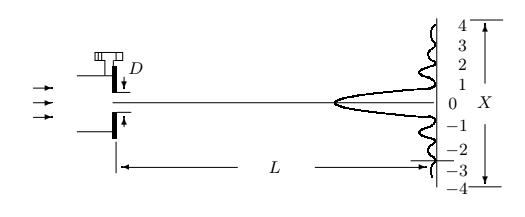
\includegraphics[width=15cm]{scheme_II.png}
    \caption{Спектр щели}
    \label{fig:scheme_II}
\end{figure}

\newpage

\subsection*{Измерения}

\begin{enumerate}
    \item Получим на удалённом экране спектр щели (рис. \ref{fig:scheme_II}). Меняя ширину щели проследим за изменением спектра на экране и оценим интервал, для которого можно наблюдать и измерять спектр.
    \item Проведем измерения ширины $m$ минимумов (центральный считается за 2) для диапазона такого диапазона ширины, как в пункте I. Занасем результаты в Таблицу 2. ($b$ в этой части отмеряется от $b_0 = 0.42$ мм)
    
    \begin{minipage}{0.5\textwidth}
        \begin{tabular}{|lllll|}
        \hline
        \multicolumn{1}{|l|}{$b$, мм} & \multicolumn{1}{l|}{$x$, см} & \multicolumn{1}{l|}{m} & \multicolumn{1}{l|}{$m/x$, 1/см} & $\sigma \frac{m}{x}$ \\ \hline
        0.05                          & 18.5                         & 2                      & 0.108                            & 0.006                 \\ \hline
        0.1                           & 12                           & 2                      & 0.167                            & 0.008                 \\ \hline
        0.15                          & 17.5                         & 4                      & 0.23                             & 0.006                 \\ \hline
        0.2                           & 14.8                         & 4                      & 0.27                             & 0.007                 \\ \hline
        0.25                          & 10.1                         & 9                      & 0.89                             & 0.01                 \\ \hline
        0.3                           & 7.8                          & 12                     & 1.53                             & 0.013                 \\ \hline
        0.35                          & 9.8                          & 22                     & 2.2                              & 0.010                 \\ \hline
        0.4                           & 7.1                          & 22                     & 3.1                              & 0.014                 \\ \hline
        0.45                          & 7.2                          & 26                     & 3.6                              & 0.014                 \\ \hline
        0.5                           & 5.6                          & 26                     & 4.6                              & 0.018                 \\ \hline
        \end{tabular}
        \captionof{table}{Ширина щели и размер диффракционной картины}
        \label{table::size}
    \end{minipage}
    \begin{minipage}{0.5\textwidth}
        \begin{center}
            \begin{tikzpicture}[scale=1]
                \begin{axis}[
                    	axis lines = middle,
                    	xlabel = {$b$, мм},
                        ylabel = {$m/x$, 1/см},
                    	ylabel style={red, scale=1},
                        xlabel style={red, scale=1},
                    	title={Зависимость диффракции от ширины щели},
                    	table/col sep=semicolon,
                    ]
            	    \addplot +[blue, only marks] plot[
        			error bars/.cd,
        			x dir = both,
        			x fixed = 0.01,
        			y dir = both,
        			y explicit relative,
        		    ] table[x=B, y=LB, y error = DLB]{diff.csv};
		            \addplot[color=red, domain=0.15:0.5]{14.37 * x - 2.70};
            	\end{axis}
            \end{tikzpicture}
        \end{center}
    \end{minipage}
    
    Опять наблюдаем неточность в определении момента открытия щели. По графику найдем точный момент открытия щели $b_{II} = 0.61мм$ и угловой коэффициент $k = 1.4$ 1/$\text{мм}^2$ $\approx \frac{1}{\lambda L} = 1.26$ 1/$\text{мм}^2$, измерив $L = 125$ см.
    
\end{enumerate}

\section*{Определение периода решёток}

\begin{enumerate}
    \itemПоставим кассету с двумерными решётками (сетками) вплотную к выходному окну лазера. Для каждой сетки измерим расстояние $X$ между $m$-ми пиками и отметим $m$ — количество пиков. Рассчитаем расстояния $\Delta X$ между соседними максимумами и определим период каждой решётки $d_с = f(\Delta X)$, используя соотношения:
        \begin{equation*}
            \Delta X=\frac{X}{m}=\frac{\lambda}{d_{\mathrm{c}}} L
        \end{equation*}
        Результаты занесем в Таблицу \ref{table::no_lenses}.
    
        \itemДалее линзу Л$_{2}$ с максимальным фокусом $\left(F_{2} = 11 \mathrm{~cm}\right)$ поставим на расстоянии $\simeq F_{2}$ от кассеты. В плоскости Ф линза Л$_{2}$ даёт Фурье-образ - сетки её спектр, а короткофокусная линза Л$_{3}\left(F_{3} = 2,5 \mathrm{~cm}\right)$ создаёт на экране увеличенное изображение этого спектра (Рис \ref{fig:scheme_III}).
        Измерим $X$ и $m$ для всех сеток, где это возможно. Так как экран достаточно удалён $\left(b_{3} \gg a_{3}\right)$, то практически $a_{3}=F_{3}$, и расстояние между линзами $\simeq F_{2}+F_{3} .$
        
        \begin{figure}[h]
            \centering
            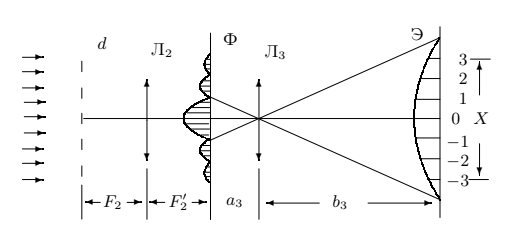
\includegraphics[width=15cm]{scheme_III.png}
            \caption{Схема лабораторной установки для наблюдения увеличенной дифракции на решетках}
            \label{fig:scheme_III}
        \end{figure}

        \itemЗная увеличение линзы ${Л_{3}}\left(\Gamma_{3}=b_{3} / a_{3}\right)$, можно рассчитать расстояние между максимумами $\Delta x$ в плоскости $\Phi$, а затем период сетки $d_{л}$ :
        $$
        \Delta x=\frac{\Delta X}{\Gamma_{3}}=\frac{\lambda}{d_{l}} F_{2}
        $$
        Занесем данные в таблицу \ref{table::with_lenses}:
\end{enumerate}


\begin{minipage}{0.5\textwidth}
    \begin{center}
    \begin{tabular}{|l|l|l|l|l|}
    \hline
    n & $X$, см & m  & $\Delta X$, мм & $d_c$, мкм \\ \hline
    1 & 14.5    & 4  & 36.3           & 21.8       \\ 
    2 & 14.7    & 6  & 24.5           & 32.3       \\ 
    3 & 14.5    & 12 & 12.1           & 65.5       \\ 
    4 & 12.0    & 20 & 6.00           & 132        \\ 
    5 & 12.5    & 24 & 4.79           & 165        \\ \hline
    \end{tabular}
    \captionof{table}{Дифракция без линз}
    \label{table::no_lenses}
    \end{center}
\end{minipage}
\begin{minipage}{0.5\textwidth}
    \begin{center}
    \begin{tabular}{|l|l|l|l|l|}
    \hline
    n & $X$, см & m  & $\Delta X$, см & $d_l$, мкм \\ \hline
    1 & 28.7    & 2  & 14.4           & 21.2       \\
    2 & 19.3    & 2  & 9.65           & 31.6       \\
    3 & 19.3    & 4  & 4.83           & 62.9       \\
    4 & 19.3    & 8  & 2.41           & 126        \\
    5 & 18.3    & 10 & 1.83           & 166        \\ \hline
    \end{tabular}
    \captionof{table}{Дифракция с линзами}
    \label{table::with_lenses}
    \end{center}
\end{minipage}
$$$$
Погрешность получившихся значений можно оценить как 
$$\sigma d_l \approx \sqrt{\left(\frac{\Delta F_2}{F_2}\right) + \left(\frac{\Delta X}{X}\right) + \left(\frac{\Delta L}{L}\right)} \approx 1\%$$

\section*{Пространственное преобразование спектров}

\begin{enumerate}
    \item Снова поставим тубус со щелью к окну лазера (рис. 4) и найдем на Экране резкое изображение щели с помощью линзы Л$_{2}\left(F_{2} = 11 \mathrm{~cm}\right) .$ В фокальной плоскости $\Phi$ линзы Л$_{2}$ поставим кассету с сетками, которые будут «рассекать» Фурье-образ щели - осуществлять пространственную фильтрацию. Подберем такую ширину входной щели $D$, чтобы на экране можно было наблюдать мультиплицированное изображение для всех сеток. Чем уже щель, тем шире её Фурье-образ и тем легче рассечь его сетками.
    
    \begin{figure}[h]
        \centering
        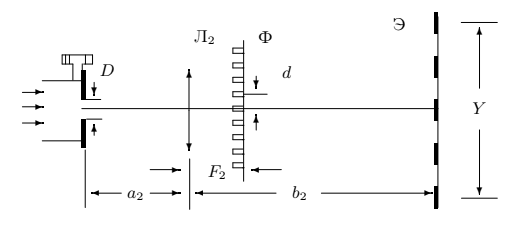
\includegraphics[width=15cm]{scheme_IV.png}
        \caption{Схема лабораторной установки рассечения Фурье-образа}
        \label{fig:scheme_IV}
    \end{figure}
    
    \newpage
    
    \item Снимем зависимость $Y$ (расстояние между удалёнными изображениями щели и и $k$ (число промежутков между изображениями) от $n$ (номер сетки) для фиксированной ширины входной щели. Данные занесем в Таблицу \ref{table::Fourier}.

    Запишем величину $D = ???$. Измерим расстояния $a_{2} = 11.8$ см и $b_{2} = 123$ см для расчёта увеличения $\Gamma_{2}$. Рассчитаем периоды $\Delta y$ «фиктивных» решёток, которые дали бы такую же периодичность на экране: $\Delta y=\Delta Y / \Gamma_{2}$, где $\Delta Y=Y / K .$

    Построим график $\Delta y=f\left(1 / d_{c}\right)$, где $d_{c}-$ периоды решёток, определённые по спектру:
        
    \begin{minipage}{0.5\textwidth}
        \centering
        \begin{tabular}{|l|l|l|l|l|}
        \hline
        n & k  & $Y$, см & $\Delta y$, мм & $1/d_l$, 1/ мм \\ \hline
        1 & 6  & 18.1    & 2.89           & 47.2           \\
        2 & 8  & 16.0    & 1.92           & 31.6           \\
        3 & 8  & 14.0    & 1.68           & 15.9           \\
        4 & 20 & 10.0    & 0.48           & 7.93           \\
        5 & 20 & 7.0     & 0.34           & 6.02           \\ \hline
        \end{tabular}
    \captionof{table}{Рассечение Фурье образа}
    \label{table::Fourier}
    \end{minipage}
    \begin{minipage}{0.5\textwidth}
        \begin{center}
            \begin{tikzpicture}[scale=1]
                \begin{axis}[
                    	axis lines = middle,
                    	xlabel = {$1/ d_l$, 1/мм},
                        ylabel = {$\Delta y$, мм},
                    	ylabel style={red, scale=1},
                        xlabel style={red, scale=1},
                    	title={Зависимость $\Delta y \left(1/d_l\right)$},
                    	table/col sep=semicolon,
                    ]
            	    \addplot +[blue, only marks] plot[
        			error bars/.cd,
        			x dir = both,
        			x fixed = 0.01,
        			y dir = both,
        			y fixed = 0,
        		    ] table[x=IDL, y=DDY]{fouri.csv};
		            \addplot[color=red, domain=5:50]{0.0616 * x - 0.0211};
            	\end{axis}
            \end{tikzpicture}
        \end{center}
    \end{minipage} 
    
    Зависимость должна быть линейной, поскольку
    $$
    \frac{\lambda}{\Delta y} F_{2}=d_{\mathrm{c}}
    $$
    
\end{enumerate}

\section{Вывод}

Мы пронаблюдали эффекты Фурье оптики такие как дифракция, рассечение изображения и фильтрация Фурье-компонент изображения.
Полученные нами результаты согласуются друг с другом:
\begin{enumerate}
    \item Двумя способами точно измерен момент открывания щели: 0.62 мм для метода геометрической оптики и 0.61 мм для дифракционного метода.
    \item Двумя способами измерены периоды решеток:
    \begin{table}[h]
        \centering
        \begin{tabular}{|l|l|l|l|l|l|}
        \hline
        $n$        & 1    & 2    & 3    & 4   & 5   \\ \hline
        $d_c$, мкм & 21.8 & 32.3 & 65.5 & 132 & 165 \\ \hline
        $d_l$, мкм & 21.2 & 31.6 & 62.9 & 126 & 166 \\ \hline
        \end{tabular}
    \end{table}
    \item Для фильтрации Фурье-образов отношения ширины щели при прямой фильтрации и под углом $45\deg$ получено отношение $\frac{0.26\text{мм}}{0.18\text{мм}} = 1.44 \approx \sqrt{2}$, как и предсказывает теория
\end{enumerate}


\end{document}